\chapter{Schwarzschild black hole}
\label{s:sch}
\index{Schwarzschild!black hole}

\minitoc

\section{Introduction}

After having discussed stationary black holes in Chap.~\ref{s:sta},
we examine here the simplest of them: the Schwarzschild black hole.
Let us recall the prime importance of the Schwarzschild black hole
in general relativity stems from the no-hair theorem (Sec.~\ref{s:sta:no-hair}),
which implies that any non-rotating black hole in an asymptotically flat
4-dimensional spacetime must a Schwarzschild black hole.

\section{Schwarzschild solution}

\subsection{Vacuum Einstein equation with a cosmological constant}

Let us search for a static and spherically symmetric solution of the
Einstein equation (\ref{e:bas:Einstein_eq}) in a vacuum
4-dimensional spacetime $(\M,\w{g})$ with some arbitrary cosmological constant
$\Lambda$. Setting $\w{T}=0$ in Eq.~(\ref{e:bas:Einstein_eq}) shows
that the equation to solve is
\be \label{e:sch:vac_Einstein_eq}
     \w{R} + \left(\Lambda - \frac{1}{2}\, R\right) \w{g} = 0 ,
\ee
$\w{R}$ being the Ricci tensor of $\w{g}$ and $R:=g^{\mu\nu} R_{\mu\nu}$ its
trace with respect to $\w{g}$, i.e. the so-called Ricci scalar
(cf. Sec.~\ref{s:bas:Ricci_tensor} in Appendix~\ref{s:bas}).
Let us first note that Eq.~(\ref{e:sch:vac_Einstein_eq}) implies a
constraint on the Ricci scalar. Indeed the trace with respect to $\w{g}$
of Eq.~(\ref{e:sch:vac_Einstein_eq}) is
\[
    R + \left(\Lambda - \frac{1}{2}\, R\right) \times 4 = 0 ,
\]
hence
\be \label{e:sch:R_4Lamb}
    \encadre{R = 4\Lambda} .
\ee
In particular the Ricci scalar is constant.
Inserting this value back into (\ref{e:sch:vac_Einstein_eq}), we get
\be \label{e:sch:vac_Einstein_eq_Lamb}
    \encadre{ \w{R} = \Lambda \, \w{g} } .
\ee
Since this equation yields to (\ref{e:sch:R_4Lamb}) as well, we conclude
that it is equivalent to (\ref{e:sch:vac_Einstein_eq}).

\subsection{Static and spherically symmetric metric}

Let us assume that the spacetime $(\M,\w{g})$
is \defin{static}\index{static spacetime}, i.e. that it is
admits a Killing vector field $\w{xi}$ that is timelike and
hypersurface-orthogonal (cf. Sec.~\ref{s:sta:staticity_thm}).
Moreover, we assume that $(\M,\w{g})$ is \defin{spherically symmetric},
i.e. that it is invariant under the action of the rotation group $\mathrm{SO}(3)$,
with spacelike orbits (cf. Sec.~\ref{s:neh:symmetries}).

\section{Maximal extension}

\begin{figure}
\centerline{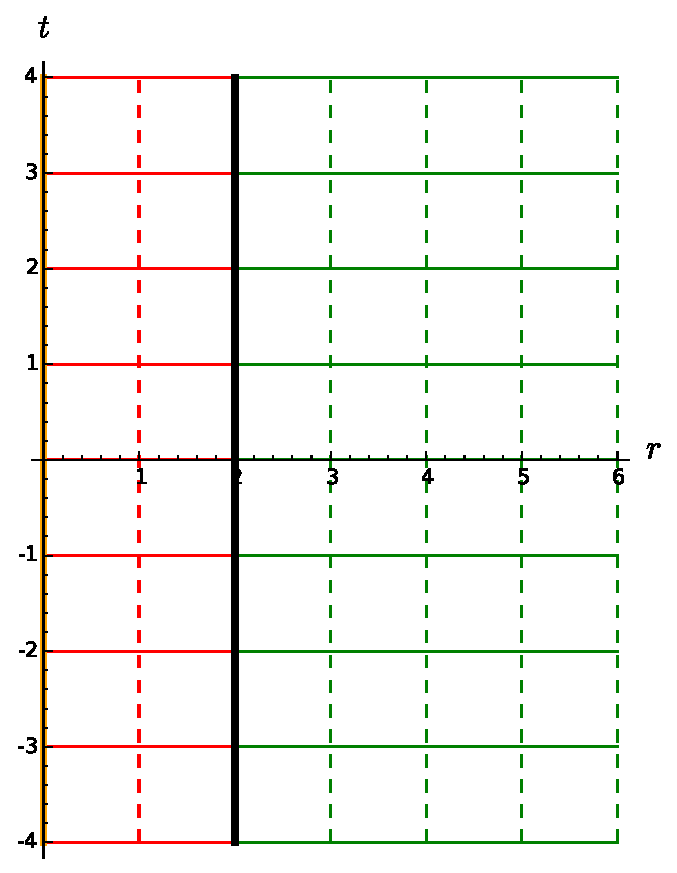
\includegraphics[height=0.37\textheight]{sch_coord_schwarz.pdf}\qquad
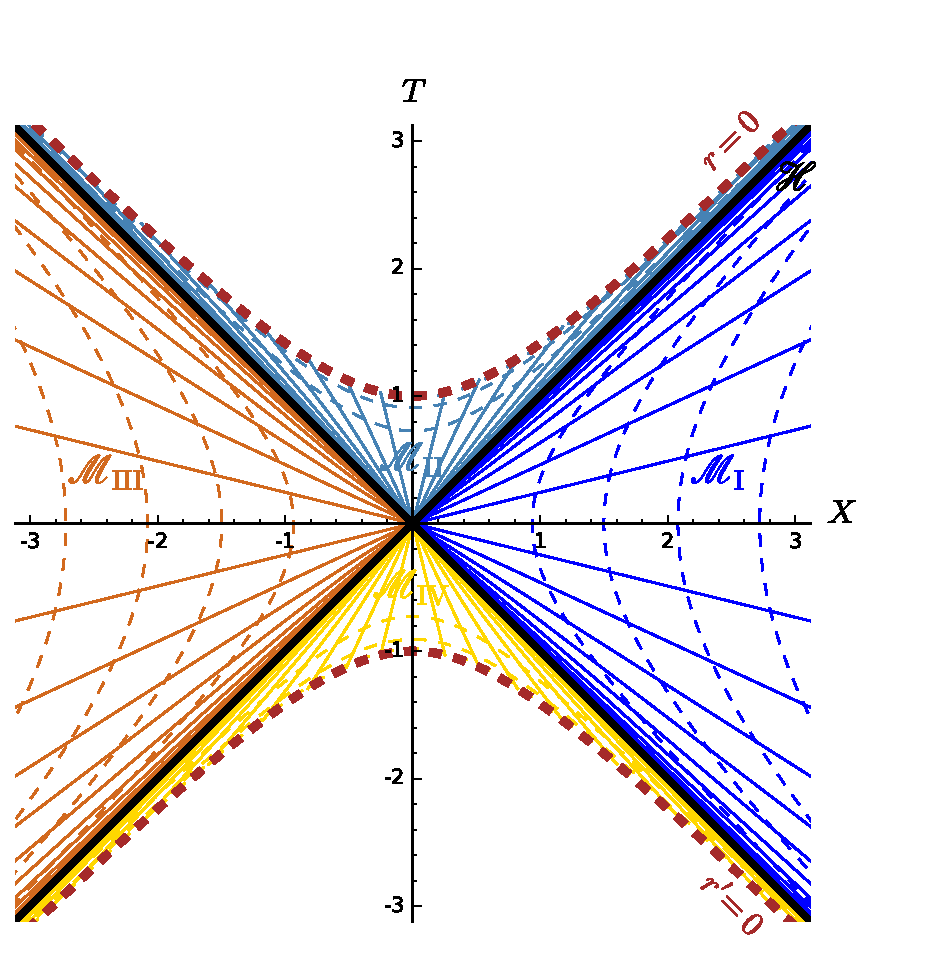
\includegraphics[height=0.37\textheight]{sch_kruskal_diag.pdf}}
\caption[]{\label{f:sch:kruskal_diag} \footnotesize
Schwarzschild spacetime depicted in Schwarzschild-Droste coordinates $(t,r)$
(left) and in Kruskal-Szekeres coordinates $(T,X)$ (right). In both figures,
green (resp. red) solid curves denote the hypersurfaces $t=\mathrm{const}$
in Region~I (resp. II), while green (resp. red) dashed curves
denote the hypersurfaces $r=\mathrm{const}$ in Region~I (resp. II).
The future and past event horizons are marked by thick black lines, while the
singularity at $r=0$ is depicted in orange. Regions III and IV are depicted
in grey and pink respectively. Note that the left figure covers only Regions I and II.}
\end{figure}

\begin{figure}
\centerline{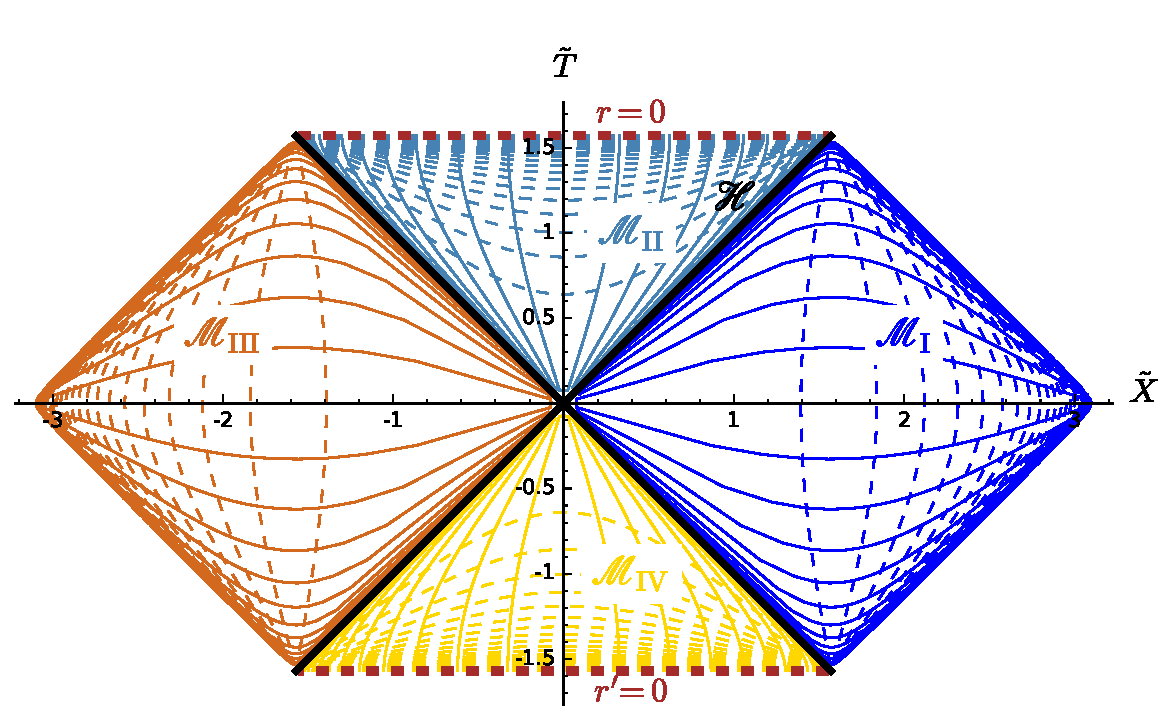
\includegraphics[width=0.9\textwidth]{sch_carter-penrose.pdf}}
\caption[]{\label{f:sch:sch_carter-penrose} \footnotesize
Schwarzschild spacetime depicted in Carter-Penrose coordinates $(\tilde{T},\tilde{X})$; the color code
is the same as in Fig.~\ref{f:sch:kruskal_diag}.
As Fig.~\ref{f:sch:kruskal_diag}, this figure has been produced with
SageManifolds (cf. Appendix~\ref{s:sam}).}
\end{figure}

